\documentclass[FM,BP]{tulthesis}

\newcommand{\verze}{2.1}

\usepackage{polyglossia}
\setdefaultlanguage{czech}


\usepackage{makeidx}
\makeindex

\usepackage{fontspec}
\usepackage{xunicode}

\usepackage{xltxtra}
\usepackage{tabularx}

\usepackage{tikz}
\usepackage{bbding}
\usepackage{graphicx}
\usepackage{float}
\usepackage{lscape}
\usepackage{nameref}
\usepackage[format=plain,
            labelfont=it,
            textfont=it]{caption}
\usepackage{amsmath}
\usepackage{listings}
\usepackage{color}
\graphicspath{ {./images}{./tex-tul-template} }

% příkazy specifické pro tento dokument / specific commands for this document
\newcommand{\argument}[1]{{\ttfamily\color{\tulcolor}#1}}
\newcommand{\argumentindex}[1]{\argument{#1}\index{#1}}
\newcommand{\prostredi}[1]{\argumentindex{#1}}
\newcommand{\prikazneindex}[1]{\argument{\textbackslash #1}}
\newcommand{\prikaz}[1]{\prikazneindex{#1}\index{#1@\textbackslash #1}}
\newcommand{\ccheckmark}{{\color[HTML]{009901} \CheckmarkBold}}
\newcommand{\ccrossmark}{{\color[HTML]{CB0000} \XSolid}}
\newenvironment{myquote}{\begin{list}{}{\setlength\leftmargin\parindent}\item[]}{\end{list}}
\newenvironment{listing}{\begin{myquote}\color{\tulcolor}}{\end{myquote}}
\clubpenalty=10000
\widowpenalty=10000
\sloppy

% deklarace pro titulní stránku / title page declaration
\TULtitle{Řešení problematiky informačního systému střední školy}{}
\TULauthor{Daniel Adámek}

% pro bakalářské, diplomové a~disertační práce / for bachelor, master theses and dissertation
\TULprogramme{B0613A140005}{Informační technologie}{Information technology}
\TULbranch{}{Aplikovaná informatika}{Applied Informatics}
%\TULbranch{1802T008}{Nějaký jiný obor}{Some other branch}
\TULsupervisor{Ing. Lenka Kosková Třísková Ph.D.}
\TULyear{2024}

% pro habilitační práce / habilitation thesis
%\TULbranch{}{Technická kybernetika}{Technical cybernetics}
%\TULyear{2022}

% Použití bibLateXu, pracuje s~ISO stylem
% BibLaTeX settings, works with ISO style
\usepackage[ 
    backend=biber
    % ,style=iso-authoryear % styl vyžaduje FZS TUL , místo příkazu \cite{} je potřeba využít \parencite{} (sazba kulatých závorek) / style required by FZS TUL use \parencite{} instead of \cite{}
    ,style=iso-numeric
    ,style=numeric
    ,sortlocale=cs_CZ
    ,autolang=other
    ,bibencoding=UTF8
    %,urldate=edtf
    ,maxcitenames=2 %maximum v~textu citovaných jmen
    ,maxbibnames=3 %maximum v~seznamu vyjmenovaných autorů
    ]{biblatex}

\addbibresource{refs.bib}% vložení seznamu literárních zdrojů v~bib formátu / input of references in bib format

% Úprava iso-numeric.bbx v~souladu s~požadavky TUL hranaté závorky v~číslovaném seznamu / Modification of iso-numeric.bbx in accordance with TUL requirements of square brackets in a~numbered list
\DeclareFieldFormat{labelnumberwidth}{\mkbibbrackets{#1}}

% Formátování podle pokynů FZS, při využití stylu iso-authoryear, čárka mezi jmény a~poslední jméno se spojkou a~/ special requirements of FZS TUL 
\DeclareDelimFormat{multinamedelim}{\addcomma\space}

\DeclareDelimFormat{finalnamedelim}{%
  \ifnumgreater{\value{liststop}}{2}{\finalandcomma}{}%
  \addspace\bibstring{and}\space}

\DeclareNameAlias{author}{family-given/given-family} 
%%%%%%%%%%%%%%%%%%%%%%%%%%

\usepackage{csquotes} %užití biblatexu hlasí warnings, důvodem může být použití českých uvozovek v~citacích! / solving of problems with Czech quotations
\urlstyle{same} %sazba url odkazů stejným fontem jako ostatní text, řešení problémů v~zalamování hypertextových odkazů v~citacích / url in references setting into the same form as text 

% Listings konfigurace
\definecolor{lightgray}{rgb}{.9,.9,.9}
\definecolor{darkgray}{rgb}{.4,.4,.4}
\definecolor{purple}{rgb}{0.65, 0.12, 0.82}

\lstdefinelanguage{JavaScript}{
  keywords={abstract, any, as, boolean, break, case, catch, class, console, 
    const, continue, debugger, declare, default, delete, do, else, enum, export, 
    extends, false, finally, for, from, function, get, if, implements, import, in, 
    infer, instanceof, interface, keyof, let, module, namespace, never, new, null, 
    number, object, package, private, protected, public, readonly, require, return, 
    set, static, string, super, switch, symbol, this, throw, true, try, type, typeof, 
    undefined, unique, unknown, var, void, while, with, yield},
  keywordstyle=\color{blue}\bfseries,
  ndkeywords={class, export, boolean, throw, implements, import, this},
  ndkeywordstyle=\color{darkgray}\bfseries,
  identifierstyle=\color{black},
  sensitive=false,
  comment=[l]{//},
  morecomment=[s]{/*}{*/},
  commentstyle=\color{purple}\ttfamily,
  stringstyle=\color{red}\ttfamily,
  morestring=[b]',
  morestring=[b]"
}

\lstset{
   language=JavaScript,
   backgroundcolor=\color{lightgray},
   extendedchars=true,
   basicstyle=\footnotesize\ttfamily,
   showstringspaces=false,
   showspaces=false,
   numbers=left,
   numberstyle=\footnotesize,
   numbersep=9pt,
   tabsize=2,
   breaklines=true,
   showtabs=false,
   captionpos=b
}



\begin{document}

% Prohlášení
\ThesisStart{male}
%\ThesisStart{zadani-a-prohlaseni.pdf}

% Abstrakt
\begin{abstractCZ}
    Tato bakalářská práce se primárně zaměřuje na návrh a implementaci nových komponent pro řešení stávajícího informačního systému střední průmyslové školy, s cílem eliminovat identifikované slabiny a využít potenciál pro zlepšení. Práce vychází z podrobné analýzy současného stavu systému, včetně jeho funkcionalit, toku dat, synchronizačních procesů, API rozhraní, legislativních požadavků a bezpečnostních opatření. Na základě zjištěných výsledků se práce soustředí na návrh a implementaci klíčových funkcí pro efektivnější správu školy a odbourání automatizovatelných a repetetivních úkonů. Důraz je kladen na praktickou aplikovatelnost navrhovaných řešení, jejich integraci do stávajícího systému a možnost dalšího rozvoje.
\end{abstractCZ}

\begin{keywordsCZ}
    informační systém, návrh, in-house vývoj, školství
\end{keywordsCZ}
    
    \vspace{2cm}
    
\begin{abstractEN}
    This bachelor thesis primarily focuses on the design and implementation of new components for the solution of the existing information system of a secondary industrial school, with the aim of eliminating identified weaknesses and exploiting the potential for improvement. The work is based on a detailed analysis of the current state of the system, including its functionalities, data flow, synchronization processes, API interfaces, legislative requirements and security measures. Based on the findings, the thesis focuses on the design and implementation of key features for more efficient school management and the elimination of automated and repetitive tasks. Emphasis is placed on the practical applicability of the proposed solutions, their integration into the existing system and the possibility of further development.
\end{abstractEN}
    
\begin{keywordsEN}
    information system, design, in-house development, education
\end{keywordsEN}

% Volná stránka
\clearpage

% Poděkování
\begin{acknowledgement}
    Prvně bych rád vyjádřil svou vděčnost Střední průmyslové škole elektrotechnické, Praha 2, Ječná 30, kterou zastupuje ředitel Ing. Bc. et Bc. Ondřej Mandík ING-PAED IGIP. Bez jeho laskavosti a podpory by toto dílo nebylo možné realizovat. Škola mi poskytla nezbytné informace, umožnila mi upravit svůj informační systém.. Tato zkušenost byla pro mě nesmírně cenná a pomohla mi v mnoha studijních i pedagogických aspektech.
    
    Zvláštní poděkování patří všem zaměstnancům školy a mým kolegům pedagogům, kteří mi pomohli kritickým pohledem na stávající systém a při hledání nových, lepších řešení. Jejich nápady a zpětná vazba byly jedním z klíčových aspektů pro vytvoření nového informačního systému, který je efektivní.
    
    Dále bych chtěl poděkovat všem členům mého vedení, rodině a přátelům, kteří mi poskytli cennou pomoc a podporu během procesu vytváření této bakalářské práce. Jejich trpělivost, porozumění a povzbuzování bylo pro mě během celého procesu klíčové.
    
    Nakonec bych chtěl vyjádřit svou vděčnost všem, kteří se na tomto díle podíleli, ať už přímo nebo nepřímo. Bez jejich kolektivního úsilí a podpory by tento projekt nebyl možný. Vaše práce a podpora byla cenná a jsem vám za to hluboce vděčný.
    
    Děkuji všem.
\end{acknowledgement}

% Obsah
\phantomsection\addcontentsline{toc}{section}{Obsah}
\tableofcontents
\clearpage

% Seznam zkratek
\begin{abbrList}
    \textbf{FM TUL} & Fakulta mechatroniky, informatiky a mezioborových studií
    Technické univerzity v~Liberci \\
    \textbf{SPŠE Ječná} & Střední průmyslová škola elektrotechnická, Praha 2, Ječná 30 \\
    \textbf{MŠMT} & Ministerstvo školství, mládeže a tělovýchovy \\
    \textbf{IS} & Informační systém \\
    \textbf{ŠIS} & Školní informační systém \\
    \textbf{OVM} & Orgán veřejné moci \\
    \textbf{NSESSS} & Národní standard pro elektronické systémy spisové služby \\
    \textbf{UCD} & User Centered Design
\end{abbrList}

% ====================================================================== %

% Představení problému

% Třídy
\chapter{Agenda tříd}
\section{Popis problému}
Implementace agendy tříd v rozvrhovém API školního systému představuje komplexní úkol, jehož řešení vyžaduje pečlivé zvážení a hluboké pochopení jak administrativních aspektů pro správu školy, tak technických. Tento problém je esenciální pro správné fungování školního systému, který musí být schopen efektivně spravovat nejen aktuální rozvrhy a třídy, ale také uchovávat historická data.

\section{Úvod do problematiky}
Školní rozvrhový systém je srdcem administrativy školy, zajišťující, že učitelé, žáci a učebny jsou správně přiděleni v rámci různých časových bloků během školního roku. Tento systém musí zvládat nejen plánování aktuálních rozvrhů, ale také uchovávání historických dat.

\section{Požadavky}
Pro lepší pochopení problému je důležité nahlédnout do širších souvislostí. Školní systém musí splňovat následující požadavky:

\begin{itemize}
    \item \textbf{Konzistence dat:} Zajištění, že data o třídách, rozvrzích a žácích jsou konzistentní napříč různými časovými obdobími.
    \item \textbf{Historická data:} Uchovávání historických záznamů pro administrativní účely.
    \item \textbf{Flexibilita:} Systém musí být schopen flexibilně reagovat na změny, jako je přechod žáků mezi třídami, změny učitelů a učeben.
\end{itemize}

V kontextu školního rozvrhového systému se agenda tříd týká správy informací o třídách, které zahrnují aktuální třídy, jejich žáky, rozvrhy, záznamy probrané látky (\ref{sec:lesson-evidence} třídnice) a absence. Systém musí být schopen všechny změny správně zaznamenat a reflektovat. Zmíněný úkol je komplikován několika faktory:

\begin{enumerate}
    \item \textbf{Horizontální přechody žáků:} Žák během studia v průběhu školního roku může změnit třídu, obor nebo třeba školu za speficických podmínek, který stanovuje školský zákon a ředitel školy.
    \item \textbf{Vertikální přechody žáků:} Žák, který nesplní zákonné požadavky pro postup do dalšího ročníku, tedy neprospěl, může být zařazen v následujícím školním roce do jiné třídy a ročník opakovat. Žák též může vzdělávání přerušit, či školu opustit.
    \item \textbf{Přerušení studia:} Žák může během probíhajícího studia požádat ředitele školy o přerušení vzdělávání. Maximální doba trvání přerušení dle zákona § 66 odst. 5 zákona č. 561/2004 Sb. školský zákon - znění od 01.01.2024 \cite{skolsky-zakon-preruseni-obyc} až na dobu dvou let s výjimkou mateřství \cite{skolsky-zakon-preruseni-materstvi}, které se řídí jiným procesem.
    \item \textbf{Administrativní a kontrolní požadavky:} Uchovávání dat pro administrativní, právní a legislativní důvody, kterým mohou být inspekce státními orgány nebo například soudy.
\end{enumerate}

Z těchto důvodů je implementace agendy tříd ve školním rozvrhovém systému složitá a vyžaduje pečlivé zvážení různých přístupů. Je důležité navrhnout systém, který bude nejen efektivní a flexibilní, ale také bude splňovat všechny uvedené požadavky. V následujících částech této kapitoly se budeme podrobněji zabývat jednotlivými návrhy implementace a jejich dopady na celkovou konzistenci a funkčnost školního systému.

\section{Návrhy implementace}
Na základě výše uvedených požadavků a kontextu jsou navrženy tři hlavní přístupy k implementaci agendy tříd v rozvrhovém API:

\begin{enumerate}
    \item \textbf{Ukládání pouze aktuálního ročníku a aktuálních rozvrhů:} Tento přístup minimalizuje datovou zátěž na serveru tím, že uchovává pouze informace o aktuálním ročníku a rozvrzích. Historická data jsou uložena na odděleném administrativním serveru.

    \begin{figure}[H]
        \centering
        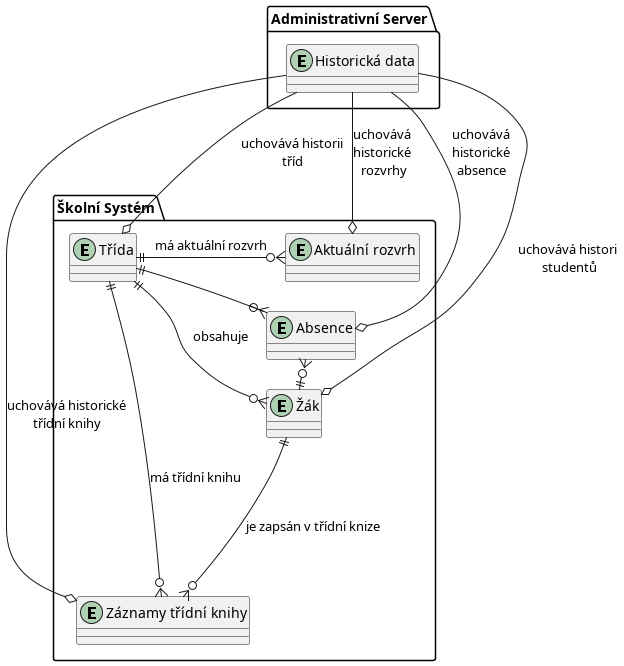
\includegraphics[width=.8\textwidth]{ed-schedule-only-actual.png}
        \caption{Diagram způsobu ukládání pouze aktuálního ročníku a aktuálních rozvrhů}
        \label{fig:ed-schedule-only-actual}
    \end{figure}
    
    Před začátkem každého školního roku by bylo tedy potřeba sjednat synchronizační proces pro archivování dat na administrativní server, smazání z rozvrhového serveru a nahrání nových dat. Tento synchronizačí mechanismus by mohl být obtížný pro správný chod. Předpokládáme, že oba servery spravuje jiný zaměstnanec. V případě chyby v programu způsobené programátory by bylo možné nenávratně přijít o důležitá data.

    \item \textbf{Třída definována prefixem, suffixem, datem vytvoření a kalkulovaným ročníkem:} Tento přístup ukládá informace o třídách pomocí kombinace prefixu, suffixu a data vytvoření třídy. Ročník je kalkulován jako rozdíl mezi datem vytvoření a začátkem aktuálního školního roku.

    \begin{figure}[H]
        \centering
        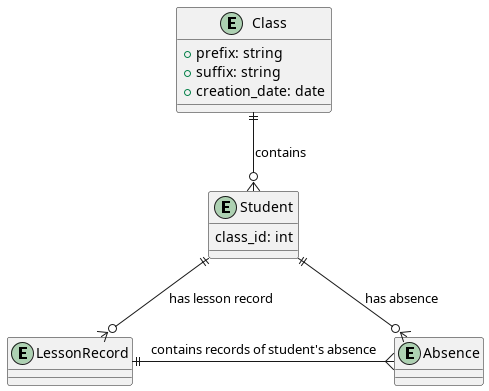
\includegraphics[width=0.7\textwidth]{ed-schedule-calculated-class.png}
        \caption{Relační schéma varianty s kalkulovaným ročníkem}
        \label{fig:ed-schedule-only-actual}
    \end{figure}

    \begin{figure}[H]
        \centering
        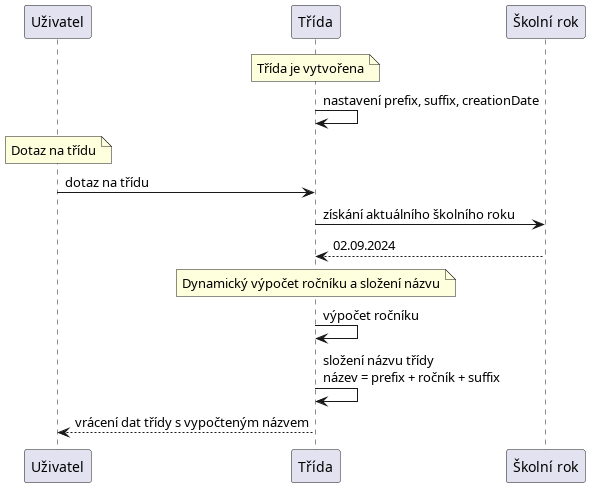
\includegraphics[width=\textwidth]{td-schedule-calculated-class.png}
        \caption{Schéma průběhu dotazu na jméno třídy}
        \label{fig:td-schedule-calculated-class}
    \end{figure}
    
    Problémem v tomto případě je samotná kalkulace. Pro dodržení aktuálnosti dat, musí být ročník vždy vypočítán, protože jakákoliv forma uchovávání mezivýsledku by mohla vést k nekonzistenci v čase. Pokud dorazí požadavek k získání aktuálních tříd, musí server vypočíst všechny ročníky a spojit celé jméno třídy.

    Dalším problémem tohoto řešení jsou propadlí nebo přecházející žáci. Jakmile žák propadne, nastávají 2 varianty řešení:
    \begin{itemize}
        \item odebrat žáka z aktuální třídy a přiřadit jej do nové třídy, ale ztratí minulé záznamy, protože třída je jedním z atributů žáka.

        Řešením může být např. psané záznamy o změnách, avšak nepokryjí všechny požadavky pro snadnou manipulaci s daty.
        \item vytvoření nového žáka, který začíná studovat v pokročilém ročníku. Tím by byla zajištěna konzistence dat, avšak duplicitní účty pro jednoho žáka.

        Řešením může být propojení minulých účtů žáka s novými (relací 1:N), kde žák by měl uložené své minulé účty. Stále je problém, že to není řešení příčiny, ale důsledku.
        \begin{figure}[H]
            \centering
            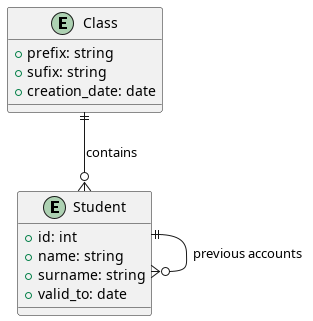
\includegraphics[width=0.5\textwidth]{ed-schedule-calculated-previous-relation.png}
            \caption{Schéma vazby na předchozí účty}
            \label{fig:ed-schedule-calculated-previous-relation}
        \end{figure}
    \end{itemize}

    \newpage
    \item \textbf{Třída definována celým názvem a datem validity od - do:}
    \label{item:class-implementation-from-to-validity} Tento přístup zahrnuje kompletní informace o třídě včetně ročníku a platnosti od-do. Každý rok se vytváří nové třídy a vztahy mezi žáky a třídami jsou zaznamenány pomocí M:N tabulky.

    \begin{figure}[H]
        \centering
        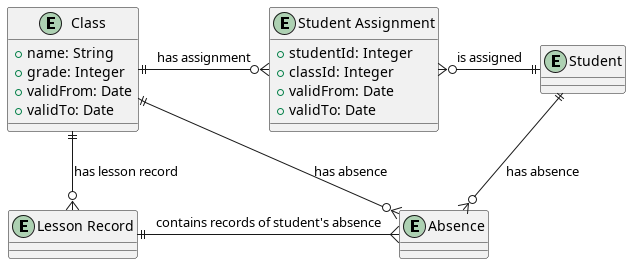
\includegraphics[width=0.9\textwidth]{ed-schedule-validity-from-to.png}
        \caption{Schéma vazby M:N pro přiřazení třídy v návrhu od - do}
        \label{fig:ed-schedule-validity-from-to}
    \end{figure}
    
    Hlavní výhodou tohoto řešení je konzistence dat i při přesunu žáků v třídách. V tom případě stačí ukončit validitu dotčených tříd, vytvořit nové se stejným názvem a přiřazení nových žáků ve správném pořadí.

    Nevýhodou je vyšší náročnost dotazování na třídu konkrétního žáka. Databáze musí projít všechny přiřazené třídy žáka, vybrat tu aktuální dle dat rozsahu dat validity a následně třídu vybrat.

    \begin{figure}[H]
        \centering
        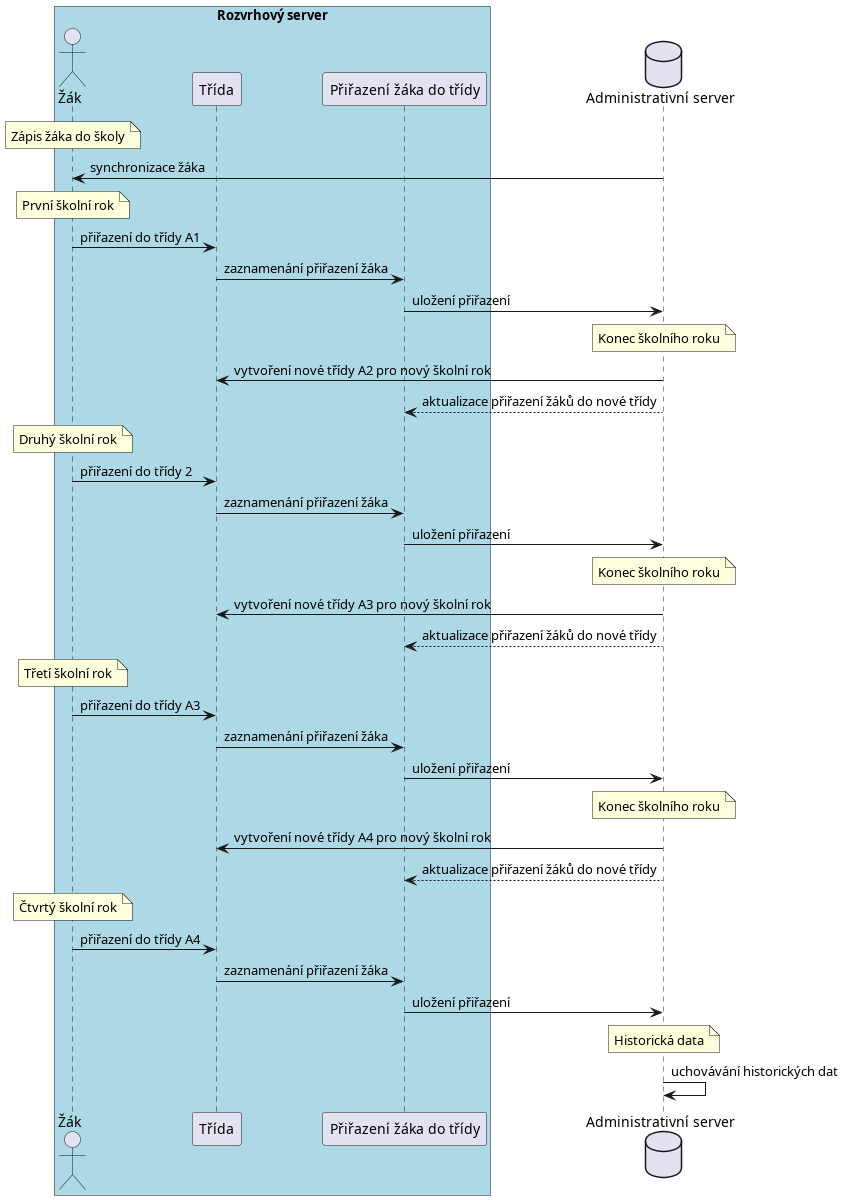
\includegraphics[width=\textwidth]{td-schedule-validity-from-to.png}
        \caption{Schéma průchodu žáka školním procesem z podlehu rozvrhů v návrhu validity od - do}
        \label{fig:td-schedule-validity-from-to}
    \end{figure}
\end{enumerate}

\section{Vyhodnocení vhodného řešení}
\begin{landscape}
    \begin{table}[H]
        \centering
        \begin{tabular}{|m{7cm}|m{7cm}|m{7cm}|}
            \hline
            \textbf{Přístup} & \textbf{Výhody (+)} & \textbf{Nevýhody (-)} \\ \hline
            \textbf{Ukládání pouze aktuálního ročníku a aktuálních rozvrhů} & 1. Minimalizuje datovou zátěž na serveru \newline 2. Jednoduché dotazování na aktuální data & 1. Nutnost synchronizačního mechanismu \newline 2. Riziko ztráty dat při chybě programu \newline 3. Vyžaduje správu od různých zaměstnanců \\ \hline
            \textbf{Třída definována prefixem, suffixem, datem vytvoření a kalkulovaným ročníkem} & 1. Snížení počtu záznamů v databázi \newline 2. Flexibilita v pojmenování tříd & 1. Komplexita kalkulace ročníků \newline 2. Potenciální nekonzistence dat \newline 3. Obtížná manipulace s propadlými nebo přecházejícími žáky \\ \hline
            \textbf{Třída definována celým názvem a datem validity od - do} & 1. Konzistence dat při přesunech žáků \newline 2. Jednoduchá správa historických záznamů \newline 3. M:N vazby umožňují flexibilní přiřazení žáků & 1. Vyšší náročnost dotazování na aktuální třídu \newline 2. Zvýšená komplexita databázových dotazů \\ \hline
        \end{tabular}
        \caption{Porovnání přístupů}
        \label{tab:class-implementation-comparison}
    \end{table}
\end{landscape}

\begin{landscape}
    \section{Vyhodnocení vhodného řešení}
    \begin{table}[H]
        \centering
        \begin{tabular}{|m{7cm}|m{7cm}|m{7cm}|}
            \hline
            \textbf{Přístup} & \textbf{Výhody (+)} & \textbf{Nevýhody (-)} \\ \hline
            \textbf{Ukládání pouze aktuálního ročníku a aktuálních rozvrhů} & 1. Minimalizuje datovou zátěž na serveru \newline 2. Jednoduché dotazování na aktuální data & 1. Nutnost synchronizačního mechanismu \newline 2. Riziko ztráty dat při chybě programu \newline 3. Vyžaduje správu od různých zaměstnanců \\ \hline
            \textbf{Třída definována prefixem, suffixem, datem vytvoření a kalkulovaným ročníkem} & 1. Snížení počtu záznamů v databázi \newline 2. Flexibilita v pojmenování tříd & 1. Komplexita kalkulace ročníků \newline 2. Potenciální nekonzistence dat \newline 3. Obtížná manipulace s propadlými nebo přecházejícími žáky \\ \hline
            \textbf{Třída definována celým názvem a datem validity od - do} & 1. Konzistence dat při přesunech žáků \newline 2. Jednoduchá správa historických záznamů \newline 3. M:N vazby umožňují flexibilní přiřazení žáků & 1. Vyšší náročnost dotazování na aktuální třídu \newline 2. Zvýšená komplexita databázových dotazů \\ \hline
        \end{tabular}
        \caption{Porovnání přístupů}
        \label{tab:class-implementation-comparison}
    \end{table}
\end{landscape}

Na základě porovnání v tabulce \ref{tab:class-implementation-comparison} je nejlepší variantou: \ref{item:class-implementation-from-to-validity}. \textbf{Třída definována celým názvem a datem validity od - do}. Tento přístup má více výhod (+) než nevýhod (-), a hlavní výhodou je jednoduchá správa historických záznamů a flexibilní vazba přiřazení žáků ke třídám a skupinám.



% Žákovské skupiny
%\chapter{Agenda žákovských skupin}

Ve vzdělávacích systémech je běžnou praxí rozdělovat studenty do tříd a následně do menších skupin pro různé předměty a aktivity, neboť tento postup významně přispívá k efektivitě vzdělávacího procesu jak pro žáky, tak pro učitele. Dělba studentů do menších skupin umožňuje přizpůsobit výuku individuálním potřebám žáků, což zvyšuje jejich zapojení a porozumění látce. Příkladně v jazykových předmětech je nezbytné vést aktivní konzultace, které jsou v menších skupinách realizovatelné mnohem efektivněji. 

Dalším důvodem pro dělení žáků je kapacitní omezení učeben, které by při výuce v rámci celého třídního kolektivu nebylo možné optimálně využít. Tato opatření vedou k vyšší kvalitě výuky a efektivnějšímu využití dostupných zdrojů.

\section{Definice}

\textbf{Class \( C \)}: třída je množina všech studentů a je označena jako \( C \). Formálně:

\[
C = \{ s_1, s_2, \ldots, s_n \}
\]

kde \( s_k \) je student a \( n \) je celkový počet studentů ve třídě.

\textbf{SubClass \( SC_{i/j} \)}: žákovská skupina (dále jen skupina) je podmnožina třídy \( C \), kde \( i \) je číslo skupiny a \( j \) je počet částí. Formálně:

\[
SC_{i/j} \subset C \quad
\]

\section{Podmínky pro skupiny}

Abychom zajistili, že žádný student není opomenut a že všechny skupiny jsou disjunktní, musí být splněny následující podmínky:

\subsection*{Úplnost}

Sjednocení všech \( j \) částí skupiny musí tvořit celou třídu \( C \):

\[
\bigcup_{i=1}^{j} SC_{i/j} = C
\]

\subsection*{Disjunkce}

Žádný student nesmí patřit do více než jedné části téže skupiny:

\[
SC_{i/j} \cap SC_{k/j} = \emptyset \quad \text{pro} \quad i \neq k
\]

\section{Kategorizace podmnožin}

V rámci tříd můžeme studenty rozdělit do různých kategorií podmnožin podle různých kritérií. Níže uvádíme několik obecných kategorií podmnožin a příklad jejich využití.

\subsection*{Dělení na zlomky}

Jedním z nejběžnějších způsobů rozdělení třídy je dělení na zlomky. Tato metoda je často využívána pro různé aktivity a předměty, kde je potřeba pracovat s menšími skupinami studentů.

\setlength{\parindent}{0em}
\setlength{\parskip}{1em}
\textbf{Příklad}: Rozdělení třídy na dvě poloviny:

\[
SC_{1/2} \quad \text{a} \quad SC_{2/2}
\]

kde:

\[
SC_{1/2} \cup SC_{2/2} = C
\]

a

\[
SC_{1/2} \cap SC_{2/2} = \emptyset
\]

Tento přístup je užitečný například při laboratorních cvičeních, kde je potřeba, aby každý student měl přístup k vybavení a učitel mohl efektivně dohlížet na práci studentů.

\subsection*{Dělení podle pohlaví}

Další běžnou metodou rozdělení studentů je podle pohlaví. Toto rozdělení může být užitečné v situacích, kde je potřeba řešit specifické potřeby studentů podle pohlaví.

\begin{samepage}
\setlength{\parindent}{0em}
\setlength{\parskip}{1em}

\textbf{Příklad}: Rozdělení třídy na dívky a chlapce:
\nopagebreak

\[
SC_{\text{dívky}} \quad \text{a} \quad SC_{\text{chlapci}}
\]
\nopagebreak

kde:
\nopagebreak

\[
SC_{\text{dívky}} \cup SC_{\text{chlapci}} = C
\]
\nopagebreak

a
\nopagebreak

\[
SC_{\text{dívky}} \cap SC_{\text{chlapci}} = \emptyset
\]

Tento přístup může být užitečný při tělesné výchově nebo v předmětech, kde jsou specifické fyziologické nebo psychologické rozdíly mezi pohlavími relevantní.
\end{samepage}

\section{Důsledky a diskuse}

\subsection*{Úplnost}

Podmínka úplnosti zajišťuje, že každý student ve třídě \( C \) je přiřazen do alespoň jedné skupiny. Pokud by některý student nebyl zahrnut v žádné skupině, nebyla by splněna podmínka:

\[
\bigcup_{i=1}^{j} SC_{i/j} \neq C
\]

To by znamenalo, že existuje alespoň jeden student \( s_k \), který nepatří do žádné části skupiny, což je nepřijatelné.
\pagebreak
\begin{samepage}
\subsection*{Disjunkce}

Podmínka disjunkce zajišťuje, že žádný student není přiřazen do více než jedné části skupiny. Pokud by některý student patřil do více než jedné části skupiny, byla by narušena disjunkčnost:
\nopagebreak

\[
SC_{i/j} \cap SC_{k/j} \neq \emptyset \quad \text{pro} \quad i \neq k
\]
\nopagebreak

To by znamenalo, že existuje alespoň jeden student \( s_k \), který patří do více než jedné části skupiny, což je také nepřijatelné.
\end{samepage}

\section{Příklady}

\subsection*{Třída a podskupiny}

Předpokládejme, že máme třídu \( C \) se \( n \) studenty:

\[
C = \{ s_1, s_2, \ldots, s_n \}
\]

Dále předpokládejme, že třídu \( C \) chceme rozdělit do \( j \) disjunktních skupin:

\[
\{ SC_{1/j}, SC_{2/j}, \ldots, SC_{j/j} \}
\]

\subsection*{Úplnost}

\[
\bigcup_{i=1}^{j} SC_{i/j} = C
\]

Tento výraz zajišťuje, že každá část skupiny je zahrnuta ve sjednocení, což pokrývá celou třídu.

\subsection*{Disjunkce}

\[
SC_{i/j} \cap SC_{k/j} = \emptyset \quad \text{pro} \quad i \neq k
\]
Tento výraz zajišťuje, že žádný student není zahrnut ve více než jedné části skupiny.

\begin{samepage}
\subsection*{Příklad pro tři části}

Pro ilustraci uvažujme třídu \( C \) se šesti studenty:
\nopagebreak
\[
C = \{ s_1, s_2, s_3, s_4, s_5, s_6 \}
\]

\noindent
Chceme třídu rozdělit do tří disjunktních skupin:

\nopagebreak

\[
\{ SC_{1/3}, SC_{2/3}, SC_{3/3} \}
\]

\noindent
Předpokládejme, že:

\nopagebreak

\[
SC_{1/3} = \{ s_1, s_2 \}
\]
\[
SC_{2/3} = \{ s_3, s_4 \}
\]
\[
SC_{3/3} = \{ s_5, s_6 \}
\]

\noindent
Poté platí:

\[
SC_{1/3} \cup SC_{2/3} \cup SC_{3/3} = \{ s_1, s_2, s_3, s_4, s_5, s_6 \} = C
\]

\noindent
a

\[
SC_{1/3} \cap SC_{2/3} = \emptyset
\]
\[
SC_{1/3} \cap SC_{3/3} = \emptyset
\]
\[
SC_{2/3} \cap SC_{3/3} = \emptyset
\]
\end{samepage}

\subsection*{Závěr}

Matematická úvaha o třídách a skupinách zajišťuje, že rozdělení studentů do skupin je úplné a disjunktní. To znamená, že každý student je přiřazen do alespoň jedné skupiny a žádný student není přiřazen do více než jedné části skupiny. Tímto způsobem je zajištěno, že žádný student není opomenut a že všechny skupiny jsou disjunktní a kompletně pokrývají celou třídu.


\section{Implementace}
V předchozí kapitole jsme diskutovali matematickou úvahu o třídách a jejich skupinách (SubClasses), kde jsme stanovili tři klíčové podmínky: úplnost, disjunkci a podmnožinovou strukturu. V této kapitole se zaměříme na implementaci těchto matematických principů do třídního a databázového modelu. Zároveň se pokusíme najít nejefektivnější řešení, které zajistí plnou konzistenci dat v databázi.

\subsection{Třídní Model}

Třídní model zahrnuje několik hlavních entit: \texttt{Class}, \texttt{SubClass}, \texttt{Student} a \texttt{StudentAssignment}. Model \texttt{Class} reprezentuje třídu jako celek, model \texttt{SubClass} reprezentuje skupiny v rámci třídy, model \texttt{Student} reprezentuje jednotlivé žáky a model \texttt{StudentAssignment} zaznamenává přiřazení žáků k třídám a skupinám.

\subsubsection*{Class}

\texttt{Class} obsahuje informace o třídě, jako jsou identifikátor třídy, označení třídy, prefix, data platnosti, kmenovou učebnu a třídního učitele. 

V této implementaci není speciálně řešena změna třídního učitele nebo kmenové učebny během školního roku. Při změně je třeba ukončit validitu staré třídy a založit novou se stejným názvem. Dojte tedy k duplikování všech vazeb žáků, tříd, skupin a rozvrhů. Tyto případy jsou zcela výjimečné a tedy není třeba situaci řešit komplikovaněji.

\subsubsection*{SubClass}

\texttt{SubClass} reprezentuje skupiny žáků v rámci třídy. Každá skupina má své vlastní identifikační číslo, název a odkaz na třídu, ke které patří. SubClass může existovat pouze v kontextu třídy, což znamená, že každá SubClass musí být vždy přiřazena konkrétní třídě.

\subsubsection*{Student}

\texttt{Student} obsahuje informace o jednotlivých žácích, jako jsou identifikační číslo, uživatelské jméno, jméno a příjmení.

\subsubsection*{StudentAssignment}

\texttt{StudentAssignment} zaznamenává přiřazení žáků k třídám a skupinám. Obsahuje odkazy na žáky, třídy a skupiny, ke kterým jsou přiřazeni. Klíčovým prvkem tohoto modelu je zajištění trvanlivosti přiřazení, tedy schopnost zaznamenávat změny přiřazení žáků v průběhu roku. 

V průběhu školního roku mohou nastat různé změny, které vyžadují aktualizaci přiřazení žáků. Tyto změny mohou zahrnovat mnoho faktorů a ty nejčastější z nich jsou vyjmenovány níže. Trvanlivost přiřazení umožňuje udržovat historický záznam o všech těchto změnách, což je nezbytné pro správu.

\textbf{Problémy a důvody pro trvanlivost:}

\begin{itemize}
    \item \textbf{Přechody mezi třídami}: Žáci mohou být během školního roku přeřazeni do jiné třídy z různých důvodů, jako jsou změny nálad v třídním kolektivu nebo přestup žáka mezi obory.
    \item \textbf{Změny ve složení skupin}: V závislosti na specifických potřebách výuky mohou být žáci přeřazeni mezi různými skupinami. Například při výuce jazyků může být potřeba změnit složení skupin kvůli homogenizaci, nebo naopak heterogenizaci skupiny, čimž v závislosti na potřebách jednotlivých žáků lze docílit zefektivnění výuky.
\end{itemize}

Model \texttt{StudentAssignment} musí být schopen zaznamenávat všechny tyto změny, aby bylo možné udržovat konzistentní a aktuální přehled o přiřazení žáků. Tento model tedy umožňuje sledování přiřazení žáků k třídám a skupinám v určitém časovém období a zajišťuje, že historické změny jsou správně zaznamenány.

\textbf{Schopnosti modelu:}

\begin{itemize}
    \item \textbf{Referenční integrita}: Každý záznam o přiřazení musí odkazovat na platné záznamy ve třídách a skupinách.
    \item \textbf{Flexibilita přiřazení}: Umožňuje přiřazení žáka buď přímo do třídy nebo do specifické skupiny.
    \item \textbf{Trvanlivost}: Udržuje historické záznamy o přiřazení, které umožňují sledovat změny v průběhu školního roku.
\end{itemize}

Tímto způsobem model \texttt{StudentAssignment} nejen zajišťuje aktuálnost a konzistenci dat, ale také poskytuje cenné historické informace, které mohou být využity pro analýzu a zlepšení vzdělávacího procesu.

\begin{figure}[H]
    \centering
    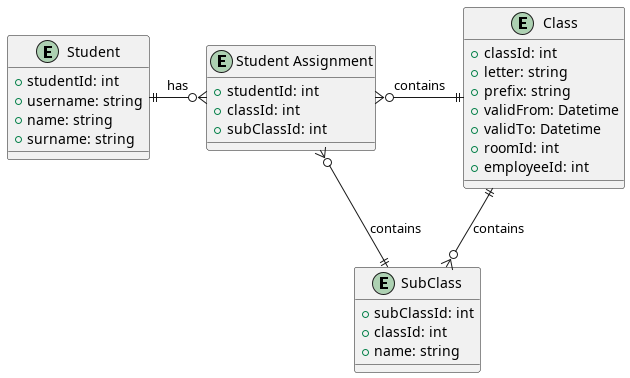
\includegraphics[width=.8\textwidth]{cd-student-assignment.png}
    \caption{Model tříd žákovských skupin}
    \label{fig:cd-student-assignment}
 \end{figure}

\subsection{Databázový Model}

Databázový model musí zajistit, že všechny podmínky úplnosti, disjunkce a podmnožinové struktury jsou dodrženy. Toho lze dosáhnout pomocí správného nastavení cizích klíčů, unikátních omezení a triggerů.

\subsubsection*{Úplnost}

Úplnost zajišťuje, že každá třída je pokryta skupinami tak, aby žádný žák nezůstal nezařazen v dané kategorii (tzn. dělení na poloviny, třetiny, dívky a chlapce). V backendové části zajistíme, že všechny skupiny dohromady pokrývají celou třídu. To můžeme kontrolovat při každém přiřazení žáka do skupiny. Je nezbytné, aby všechny skupiny dané kategorie třídy byly disjunktní a jejich sjednocení tvořilo celou třídu.

\subsubsection*{Disjunkce}

Disjunkci zajistíme na úrovni databáze pomocí unikátních omezení. Každý žák může patřit pouze do jedné skupiny určitého typu v dané třídě. To lze implementovat pomocí unikátních indexů nebo pomocí aplikační logiky, která před přiřazením žáka do skupiny provede potřebné kontroly.

\subsubsection*{Podmnožinová struktura}

Podmnožinovou strukturu zajistíme pomocí cizích klíčů a referenční integrity. Každá skupina musí odkazovat na existující třídu a každé přiřazení žáka do skupiny musí odkazovat na existujícího žáka, třídu a skupinu.

\subsection{Validace dat v aplikační logice}

Validace dat je důležitým aspektem jakéhokoliv robustního informačního systému. V tomto návrhu  systému zajišťuje validace dat konzistenci a integritu uložených informací. Níže jsou popsány validátory použité v aplikační logice.

\subsubsection*{Úvod do validace dat}

Validace dat je proces ověřování, zda vstupní data splňují stanovené požadavky a pravidla. Tato pravidla mohou zahrnovat různé aspekty, jako je formát, rozsah, konzistence a vztahy mezi jednotlivými datovými poli. Ve školním systému je validace dat implementována na úrovni aplikační logiky. To zajišťuje, že pouze správně formátovaná a platná data jsou ukládána do databáze.

V této aplikaci je použito několik validátorů, které kontrolují různé aspekty vstupních dat. Každý validátor je navržen tak, aby ověřil konkrétní sadu pravidel a zajistil, že data jsou konzistentní a správná.

\subsubsection*{Validátor dat třídy (\texttt{validateClassDates})}

Validátor \texttt{validateClassDates} je zodpovědný za ověření, zda datum začátku (\texttt{validFrom}) třídy je dříve než datum konce (\texttt{validTo}). Zajišťuje, že žádná třída nemůže mít začátek po svém konci, což by bylo nelogické a mohlo by vést k chybám při dalších operacích.

\begin{lstlisting}[title=Kód validátoru dat třídy]
function validateClassDates(instance: Class) {
    if (new Date(instance.validFrom) > new Date(instance.validTo)) {
        throw new Error('validFrom must be less than validTo');
    }
}
\end{lstlisting}

\subsubsection*{Validátor unikátnosti názvu třídy (\texttt{validateClassName})}

Validátor \texttt{validateClassName} ověřuje, že jméno třídy je unikátní v daném období platnosti. Tím je zajištěno, že nemůže existovat více tříd se stejným jménem v tomtéž období. Tím validátor předchází duplicitě názvů tříd, což by mohlo vést ke zmatkům a chybám v rozvrhu a přiřazení studentů.

\begin{lstlisting}[title=Kód validátoru unikátnosti názvu třídy]
async function validateClassName(instance: Class) {
    const existingClass = await Class.findOne({
        where: {
            name: instance.name,
            validFrom: { [Op.lte]: instance.validTo },
            validTo: { [Op.gte]: instance.validFrom }
        }
    });

    if (existingClass) {
        throw new Error('Class name already exists in the given period');
    }
}
\end{lstlisting}

\subsubsection*{Validátor časových intervalů tříd (\texttt{validateClassInterval})}

Validátor \texttt{validateClassInterval} zajišťuje, že nově vytvářená nebo aktualizovaná třída nemá časový interval, který by se překrýval s jinou třídou se stejným jménem, místností nebo učitelem. Tím zajišťuje, že třídy nebudou mít překrývající se časové intervaly, což by mohlo způsobit problémy s plánováním.

\newpage
\begin{lstlisting}[title=Kód validátoru časových intervalů tříd]
async function validateClassInterval(instance: Class) {
    const existingClass = await Class.findOne({
        where: {
          name: instance.name,
          roomId: instance.roomId,
          employeeId: instance.employeeId,
          validFrom: { [Op.lte]: instance.validTo },
          validTo: { [Op.gte]: instance.validFrom },
          classId: { [Op.ne]: instance.classId }
        }
      });
    
      if (existingClass) {
        throw new Error('Class interval is overlapping with another class');
      }
}
\end{lstlisting}

\subsubsection*{Validátor existence učitele (\texttt{validateTeacherExistence})}

Validátor \texttt{validateTeacherExistence} kontroluje, zda zaměstnanec, který je přiřazen k třídě, skutečně existuje v databázi a je učitel. Tím je zajištěno, že nejsou přiřazováni neexistující učitelé nebo nepedagogičtí zaměstnanci.

\begin{lstlisting}[title=Kód validátoru existence učitele]
async function validateTeacherExistence(instance: Class) {
    const teacher = await Employee.findOne({
        where: { employeeId: instance.employeeId, isTeacher: true }
      });
    
      if (!teacher) {
        throw new Error('Teacher does not exist');
      }
}
\end{lstlisting}

\subsubsection*{Validátor rozvrhu učitele (\texttt{validateEmployeeSchedule})}

Validátor \texttt{validateEmployeeSchedule} zajišťuje, že učitel nemá přiřazen více tříd ve stejném časovém období. Tím zajišťuje konflikty v rozvrzích učitelů.

\newpage
\begin{lstlisting}[title=Kód validátoru rozvrhu učitele]
async function validateEmployeeSchedule(instance: Class) {
    const existingTeacher = await Class.findOne({
        where: {
            employeeId: instance.employeeId,
            validFrom: { [Op.lte]: instance.validTo },
            validTo: { [Op.gte]: instance.validFrom },
            classId: { [Op.ne]: instance.classId }
        }
    });

    if (conflictingClass) {
        throw new Error('Teacher is already assigned to another class in this period');
    }
}
\end{lstlisting}

\subsubsection*{Validátor existence místnosti (\texttt{validateRoomExistence})}

Podobně jako validátor existence učitele, validátor \texttt{validateRoomExistence} ověřuje, že místnost přiřazená k třídě existuje v databázi a je učebnou. Zajišťuje, že místnost není například kancelář.

\begin{lstlisting}[title=Kód validátoru existence místnosti]
async function validateRoomExistence(instance: Class) {
    const room = await Room.findOne({ 
        where: { 
            roomId: instance.roomId,
            type: 'classroom'
        } 
    });
    
    if (!room) {
        throw new Error('Room does not exist');
    }
}
\end{lstlisting}

\subsubsection*{Validátor rozvrhu místnosti (\texttt{validateRoomSchedule})}

Validátor \texttt{validateRoomSchedule} ověřuje, že místnost není přiřazena více třídám ve stejném časovém období. Tím je zajištěno, že místnost může být kmenovou učebnou a místnost není přiřazena k více třídám zároveň.

\newpage
\begin{lstlisting}[title=Kód validátoru rozvrhu místností]
async function validateRoomSchedule(instance: Class) {
    const existingRoom = await Class.findOne({
        where: {
          roomId: instance.roomId,
          validFrom: { [Op.lte]: instance.validTo },
          validTo: { [Op.gte]: instance.validFrom },
          classId: { [Op.ne]: instance.classId }
        }
    });
    
    if (existingRoom) {
        throw new Error(
          'Room is already assigned to another class within the validity period'
        );
    }
}
\end{lstlisting}

\subsection{Diskuse o efektivitě řešení}

Pro zajištění úplné konzistence dat v databázi je nutné implementovat následující mechanismy.

\subsubsection*{Validace na úrovni aplikace}

Při každém přiřazení žáka do skupiny zkontrolujeme, zda přiřazení splňuje podmínky úplnosti a disjunkce. Pokud podmínky nejsou splněny, přiřazení se neprovede a uživatel obdrží příslušnou chybovou zprávu. Aplikační logika bude muset zohlednit také případy, kdy se celá třída učí společně a není třeba přiřazovat žáky do skupin.

\subsubsection*{Unikátní omezení}

Na úrovni databáze zavedeme unikátní omezení, která zajistí, že každý žák může patřit pouze do jedné skupiny určitého typu v dané třídě. Tím zajistíme disjunkci dat.

\subsubsection*{Referenční integrita}

Pomocí cizích klíčů zajistíme, že každá skupina je podmnožinou existující třídy a každé přiřazení žáka odkazuje na existujícího žáka, třídu a skupinu. Tím zajistíme podmnožinovou strukturu.

Implementace výše uvedených mechanismů v kombinaci s aplikační logikou poskytuje robustní řešení pro správu tříd a jejich skupin. Validace na úrovni aplikace umožňuje flexibilitu a zajišťuje, že jsou splněny všechny kladené podmínky. Unikátní omezení a referenční integrita na úrovni databáze zajišťují konzistenci dat a minimalizují riziko chyb.

Tímto způsobem zajišťujeme:

\begin{itemize}
    \item \textbf{Úplnost}: Každá třída je kompletně pokryta skupinami a žádný žák nezůstane nezařazen.
    \item \textbf{Disjunkce}: Každý žák může být přiřazen pouze do jedné skupiny určitého typu v dané třídě.
    \item \textbf{Podmnožinová struktura}: Každá skupina je vždy podmnožinou konkrétní třídy, ke které patří.
\end{itemize}

% Třídnice
\chapter{Rozvrh}
\section{Popis problému}
\section{Úvod do problematiky}
\section{Požadavky}
\section{Návrh implementace}


% ====================================================================== %

% Reference
\chapter{Reference}
\printbibliography[heading=none]

% Přílohy
\chapter{Přílohy}
\begin{itemize}
  \item Analýza pro proces modernizace školního informačního systému pro střední školu, Daniel Adámek
\end{itemize}

\end{document}
